\documentclass{anstrans}
%%%%%%%%%%%%%%%%%%%%%%%%%%%%%%%%%%%
\title{Implementation of the SP3 equations in a MOOSE-based application}
\author{Roberto E. Fairhurst Agosta, Kathryn D. Huff}

\institute{
University of Illinois at Urbana-Champaign, Dept. of Nuclear, Plasma, and Radiological Engineering\\
ref3@illinois.edu
}

%%%% packages and definitions (optional)
\usepackage{graphicx} % allows inclusion of graphics
\usepackage{booktabs} % nice rules (thick lines) for tables
\usepackage{microtype} % improves typography for PDF
\usepackage{xspace}
\usepackage{tabularx}
\usepackage{floatrow}
\usepackage{subcaption}
\usepackage{enumitem}
\usepackage{placeins}
\usepackage{amsmath}
\usepackage[acronym,toc]{glossaries}
\newacronym{ANL}{ANL}{Argonne National Laboratory}
\newacronym{API}{API}{Application Programming Interface}
\newacronym{B4C}{B4C}{boron carbide}
\newacronym{BC}{BC}{boundary condition}
\newacronym{BOC}{BOC}{beginning of the equilibrium cycle}
\newacronym{BSD}{BSD}{Berkeley Software Distribution}
\newacronym{BWR}{BWR}{Boiling Water Reactor}
\newacronym{CAISO}{CAISO}{California ISO}
\newacronym{CAPP}{CAPP}{Core Analyzer for Pebble and Prism type VHTRs}
\newacronym{CEA}{CEA}{Commissariat a l'Energie Atomique}
\newacronym{CFD}{CFD}{computational fluid dynamics}
\newacronym{CO2}{CO$_2$}{carbon dioxide}
\newacronym{CR}{CR}{control rod}
\newacronym{CRP}{CRP}{Coordinated Research Project}
\newacronym{CZP}{CZP}{Cold Zero Power}
\newacronym{DCC}{DCC}{depressurized conduction cool-down}
\newacronym{DOE}{DOE}{Department of Energy}
\newacronym[\glslongpluralkey={degrees of freedom}]{DoF}{DoF}{degree of freedom}
\newacronym{EOC}{EOEC}{end of the equilibrium cycle}
\newacronym{FCEV}{FCEV}{Fuel Cell Electric Vehicle}
\newacronym{FDM}{FDM}{Finite Difference Method}
\newacronym{FEM}{FEM}{Finite Element Method}
\newacronym{FVM}{FVM}{Finite Volume Method}
\newacronym[\glslongpluralkey={greenhouse gases}]{GHG}{GHG}{greenhouse gas}
\newacronym{GRS}{GRS}{Gesellschaft für Anlagen und Reaktorsicherheit}
\newacronym{GT-MHR}{GT-MHR}{Gas Turbine-Modular Helium Reactor}
\newacronym{H2}{H$_2$}{hydrogen}
\newacronym{He}{He}{helium}
\newacronym{HFP}{HFP}{Hot Full Power}
\newacronym{HPCC}{HPCC}{high-pressure conduction cool-down}
\newacronym{HTE}{HTE}{High-Temperature Electrolysis}
\newacronym{HTGR}{HTGR}{High-Temperature Gas-Cooled Reactor}
\newacronym{HTR}{HTR}{High Temperature Reactor}
\newacronym{HTTR}{HTTR}{High-Temperature engineering Test Reactor}
\newacronym{HZDR}{HZDR}{Helmholtz-Zentrum Dresden-Rossendorf}
\newacronym{IAEA}{IAEA}{International Atomic Energy Agency}
\newacronym{icap}{iCAP}{Illinois Climate Action Plan}
\newacronym{INL}{INL}{Idaho National Laboratory}
\newacronym{IPyC}{IPyC}{inner pyrolytic carbon}
\newacronym{JFNK}{JFNK}{Jacobian-Free Newton-Krylov}
\newacronym{KAERI}{KAERI}{Korea Atomic Energy Research Institute}
\newacronym{Keff}{k$_{eff}$}{multiplication factor}
\newacronym{LBP}{LBP}{Lumped Burnable Poison}
\newacronym{LGPL}{LGPL}{Lesser GNU Public License}
\newacronym{LOCA}{LOCA}{loss of coolant accident}
\newacronym{LPCC}{LPCC}{low-pressure conduction cool-down}
\newacronym{LTE}{LTE}{Low-Temperature Electrolysis}
\newacronym{LWR}{LWR}{Light Water Reactor}
\newacronym{MC}{MC}{Monte Carlo}
\newacronym{MHTGR}{MHTGR}{Modular High-Temperature Gas-Cooled Reactor}
\newacronym{MMR}{MMR}{Micro Modular Reactor}
\newacronym{MOC}{MOC}{middle of the equilibrium cycle}
\newacronym{MOX}{MOX}{mixed-oxide}
\newacronym{MOOSE}{MOOSE}{Multi-physics Object-Oriented Simulation Environment}
\newacronym{MPI}{MPI}{Message Passing Interface}
\newacronym{MSR}{MSR}{Molten Salt Reactor}
\newacronym{MTD}{MTD}{Champaign-Urbana Mass Transit District}
\newacronym{NEA}{NEA}{Nuclear Energy Agency}
\newacronym{NEM}{NEM}{Nodal Expansion Method}
\newacronym{NGNP}{NGNP}{Next Generation Nuclear Power}
\newacronym{NRC}{NRC}{Nuclear Regulatory Commission}
\newacronym{NSC}{NSC}{Nuclear Science Committee}
\newacronym{OECD}{OECD}{Organisation for Economic Co-operation and Development}
\newacronym{OPyC}{OPyC}{outer pyrolytic carbon}
\newacronym{ORNL}{ORNL}{Oak Ridge National Laboratory}
\newacronym{OS}{OS}{Operator-Splitting}
\newacronym{PBMR}{PBMR}{Pebble Bed Modular Reactor}
\newacronym{PDE}{PDE}{Partial Differential Equation}
\newacronym{PMR}{PMR}{Prismatic Modular Reactor}
\newacronym{PV}{PV}{photovoltaics}
\newacronym{RPV}{RPV}{Reactor Pressure Vessel}
\newacronym{RSC}{RSC}{Reserve Shutdown Control}
\newacronym{RSD}{RSD}{Relative Standard Deviation}
\newacronym{SD}{SD}{Standard Deviation}
\newacronym{SI}{SI}{Sulfur-Iodine}
\newacronym{SiC}{SiC}{silicon carbide}
\newacronym{SMR}{SMR}{Small Modular Reactor}
\newacronym{SNU}{SNU}{Seoul National University}
\newacronym{SOEC}{SOEC}{Solid Oxide Electrolysis Cells}
\newacronym{SP3}{SP$_3$}{Simplified P$_3$}
\newacronym{TIP}{TIP}{transverse integration procedure}
\newacronym{TRISO}{TRISO}{Tristructural Isotropic}
\newacronym{UIUC}{UIUC}{University of Illinois at Urbana-Champaign}
\newacronym{UNIST}{UNIST}{Ulsan National Institute of Science and Technology}
\newacronym{UK}{UK}{United Kingdom}
\newacronym{UMICH}{UMICH}{University of Michigan}
\newacronym{US}{US}{United States}
\newacronym{USNC}{USNC}{Ultra Safe Nuclear Corporation}
\newacronym{VHTR}{VHTR}{Very High-Temperature Gas-Cooled Reactor}
%\newacronym{<++>}{<++>}{<++>}
%\newacronym{<++>}{<++>}{<++>}

\makeglossaries

\usepackage[printwatermark]{xwatermark}
\usepackage{xcolor}
\usepackage{graphicx}
\usepackage{lipsum}

\newcommand{\SN}{S$_N$}
\renewcommand{\vec}[1]{\bm{#1}} %vector is bold italic
\newcommand{\vd}{\bm{\cdot}} % slightly bold vector dot
\newcommand{\grad}{\vec{\nabla}} % gradient
\newcommand{\ud}{\mathop{}\!\mathrm{d}} % upright derivative symbol

\newcolumntype{c}{>{\hsize=.56\hsize}X}
\newcolumntype{b}{>{\hsize=.7\hsize}X}
\newcolumntype{s}{>{\hsize=.74\hsize}X}
\newcolumntype{f}{>{\hsize=.1\hsize}X}
\newcolumntype{a}{>{\hsize=.45\hsize}X}
%\usepackage[pagestyles]{titlesec}
%\titleformat*{\subsection}{\normalfont}
%\titleformat{\section}{\bfseries}{Item \thesection.\ }{0pt}{}

%\newwatermark[allpages,color=gray!50,angle=45,scale=3,xpos=0,ypos=0]{DRAFT}

\begin{document}
%%%%%%%%%%%%%%%%%%%%%%%%%%%%%%%%%%%%%%%%%%%%%%%%%%%%%%%%%%%%%%%%%%%%%%%%%%%%%%%%

\section{Abstract}

\textit{

}

\section{Introduction}

% what am I doing


% lit - review: the SPN approximation
The $P_N$ method \cite{davidson_neutron_1957} discretizes the transport equation by expanding the angular dependence of the neutron flux in spherical harmonics, considering up to order $N$ polynomials.
If $N \rightarrow \infty$, the solution of the $P_N$ equations tends to the exact transport solution.
In three-dimensional geometries, the number of $P_N$ equations is proportional to $(N+1)^2$, whereas, in one-dimensional planar geometries, the number of $P_N$ equations is $(N+1)$.
Gelbard \cite{gelbard_spherical_1960} proposed the $SP_N$ approximation by replacing the second derivatives in the one-dimensional planar $P_N$ equations with three-dimensional Laplacian operators.
This approximation considerably reduces the number of equations conserving a reasonable accuracy.


Although Gelbard proposed the $SP_N$ approximation in the 60s, the method did not have a strong theoretical basis until the 90s with Pomraning \cite{pomraning_asymptotic_1993}, Brantley, and Larsen's \cite{brantley_simplifiedP3_2000} contribution.


The disadvantage of the $SP_N$ approximation is that the solution does not usually converge to the true transport solution as $N \rightarrow \infty$.

The $SP_N$ equations yield asymptotic solutions of the transport equation in a physical regime in which diffusion theory is the leading-order approximation.



However, several results \cite{mui_modified_1987} \cite{beckert_development_2007} \cite{fliscounakis_potential_2012} \cite{ryu_finite_2013} \cite{khosravi_mirzaee_reactor_2019} show that the $SP_N$ approximation yields more accurate solutions than the diffusion approximation with considerably less computational expense than the discrete ordinates ($S_N$) method.


% why is SP3 preferred over diffusion



% lit - review: software using the SPN approximation
Currently, different software uses the SP3 approximation to solve the neutron transport equation, such as SCOPE2 \cite{tatsumi_object-oriented_2002}, PARCS \cite{downar_parcs_2004}, DYN3D \cite{beckert_development_2007}, SIMULATE-5 \cite{bahadir_studsviks_2009}, and COCAGNE \cite{fliscounakis_potential_2012}.


% something about MOOSE


\section{Methodology}

% equations


\section{Results}

\subsection{C5 MOX Benchmark}

OECD/NEACRP-L-336 C5 MOX fuel benchmark \cite{cavarec_benchmark_1994}

% why is SP3 preferred over diffusion: maybe move to intro ??
MOX fuel assemblies have higher thermal absorption and fission cross-sections than UO$_2$ fuel assemblies.
Consequently, the thermal flux is lower while the power production higher.
Modeling these characteristics of reactors using MOX fuel using the diffusion approximation may be challenging.

% benchmark specification ?

Figure \ref{fig:bench1}

Figures \ref{fig:bench2} and \ref{fig:bench3} display the geometry of each type of fuel assembly.

\begin{figure}[htbp!] %or H 
    \centering
    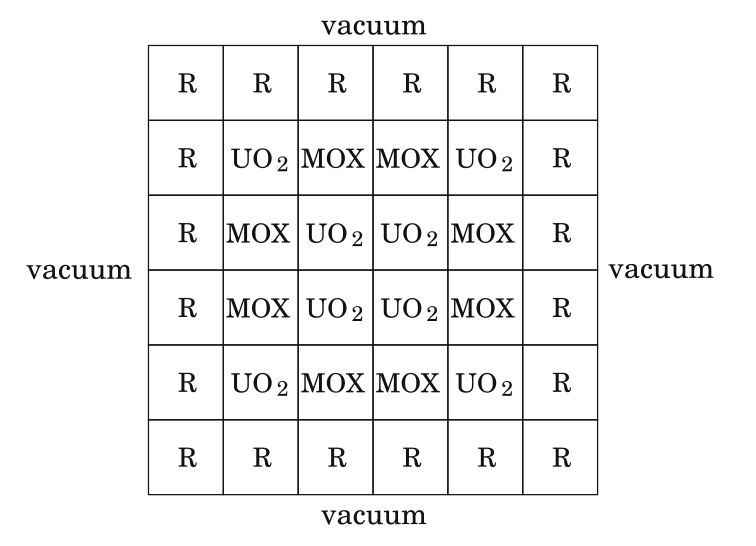
\includegraphics[width=0.95\linewidth]{figures/bench-config.png}
    \hfill
    \caption{C5 MOX benchmark configuration. \textit{R} correponds to the reflector region. Image reproduced from \cite{capilla_applications_2009}.}
    \label{fig:bench1}
\end{figure}

\begin{figure}[htbp!] %or H 
    \centering
    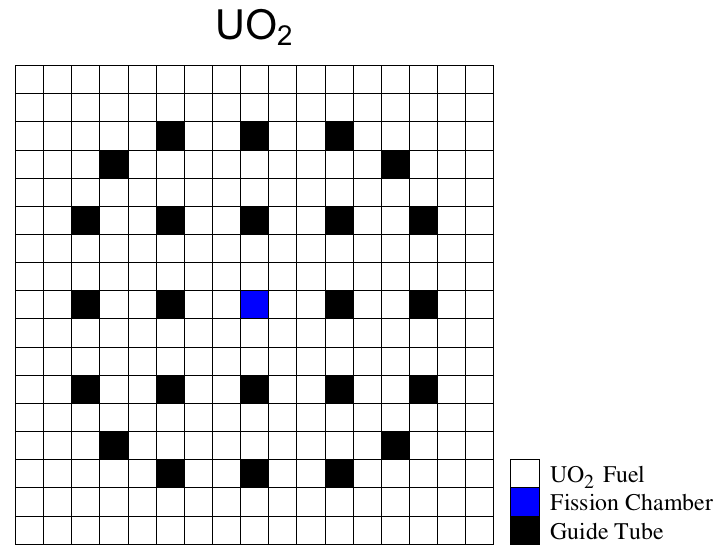
\includegraphics[width=0.95\linewidth]{figures/bench-config2.png}
    \hfill
    \caption{Structure of the UO$_2$ assembly. Image reproduced from \cite{capilla_applications_2009}.}
    \label{fig:bench2}
\end{figure}

\begin{figure}[htbp!] %or H 
    \centering
    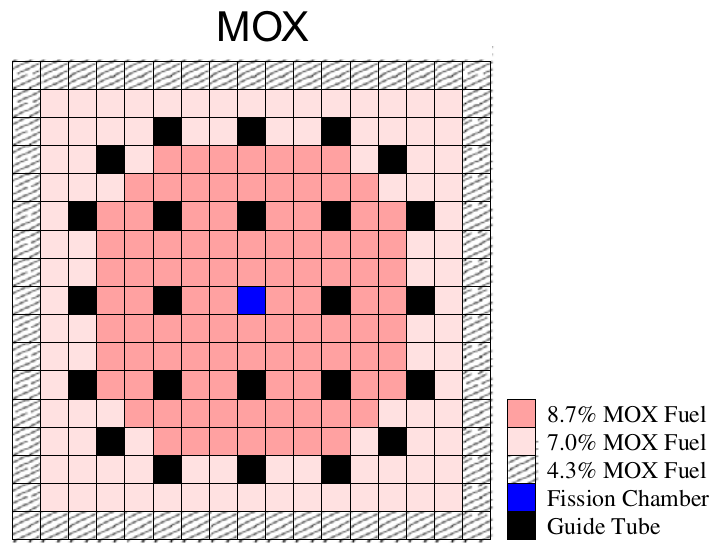
\includegraphics[width=0.95\linewidth]{figures/bench-config3.png}
    \hfill
    \caption{Structure of the MOX assembly. Image reproduced from \cite{capilla_applications_2009}.}
    \label{fig:bench3}
\end{figure}

% % \usepackage{booktabs}
% \begin{table}[]
% 	\centering
%     \caption{\gls{GGE}, \gls{DGE}, and CO$_2$ produced.}
%     \label{tab:meth}
% 	\begin{tabular}{l|lll}
% 	\toprule
% 	                 & Hydrogen & Gasoline    & Diesel      \\
% 	\midrule
% 	GGE              & 1 kg     & 1 gallon    & 0.88 gallon \\
% 	DGE              & 1.13 kg  & 1.13 gallon & 1 gallon    \\
%     CO$_2$ produced  & -        & 19.64 lbs   & 22.38 lbs   \\
%     \bottomrule
% 	\end{tabular}
% \end{table}

\section{Conclusions}



\section{Acknowledgements}

% Not sure about this
Roberto E. Fairhurst Agosta and Prof. Huff are supported by the \gls{NRC} Faculty Development Program (award NRC-HQ-84-14-G-0054 Program B).
Prof. Huff is also supported by the Blue Waters sustained-petascale computing project supported by the National Science Foundation (awards OCI-0725070 and ACI-1238993) and the state of Illinois, the DOE ARPA-E MEITNER Program (award DE-AR0000983), the DOE H2@Scale Program (award), and the International Institute for Carbon Neutral Energy Research (WPI-I2CNER), sponsored by the Japanese Ministry of Education, Culture, Sports, Science and Technology.

%%%%%%%%%%%%%%%%%%%%%%%%%%%%%%%%%%%%%%%%%%%%%%%%%%%%%%%%%%%%%%%%%%%%%%%%%%%%%%%%
\bibliographystyle{ans}
\bibliography{bibliography}
\end{document}

% \begin{figure}[htbp!] %or H 
%     \centering
%     \includegraphics[width=0.95\linewidth]{figures/radial-layout.png}
%     \hfill
%     \caption{Core radial layout. Image reproduced from \cite{oecd_nea_benchmark_2017}.}
%     \label{fig:radial}
% \end{figure}

% \begin{align}
%     \frac{1}{v_g}\frac{\partial}{\partial t} \phi_g &= \nabla \cdot D_g
%     \nabla \phi_g - \Sigma_g^r \phi_g \sum_{g \ne g'}^G
%     \Sigma_{g'\rightarrow g}^s \phi_{g'} \label{eq:diffusion}
%     \intertext{where}
%     C_i &= \mbox{concentration of delayed neutron precursors} \notag \\
%     &\phantom{{}=1} \mbox{in precursor group $i$}.
% \end{align}
